% Vektorgrafiken ausschließlich für die Lesefassung.
\definecolor{mogblue}{RGB}{34,92,133}
\definecolor{mogred}{RGB}{163,49,45}
\definecolor{mogshade}{RGB}{226,237,244}

\newcommand{\MogReserveDiagram}{%
  \par\medskip\noindent
  \begin{minipage}{\linewidth}
  \centering
  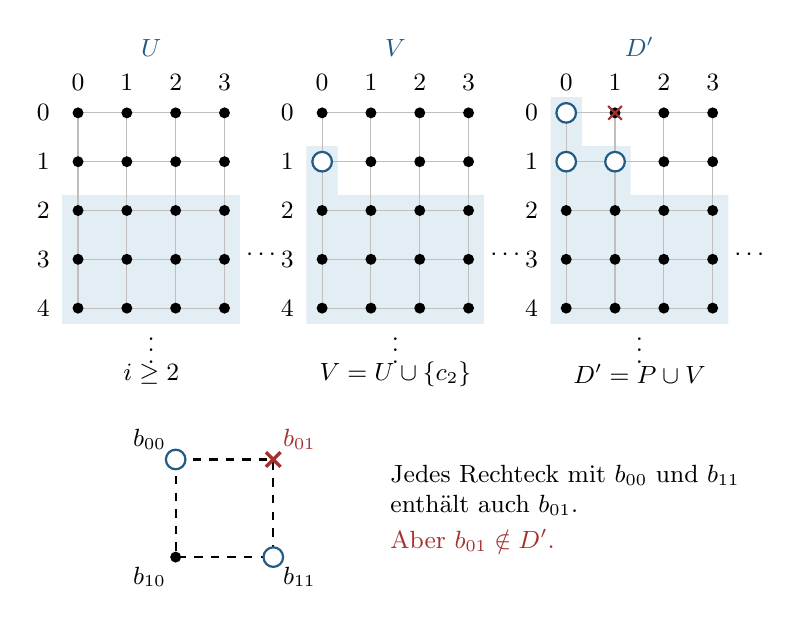
\begin{tikzpicture}[x=.62cm,y=.62cm,font=\small,
    dot/.style={circle,fill=black,inner sep=1.4pt},
    marked/.style={circle,draw=mogblue,fill=white,thick,inner sep=2.5pt}]
    % Gleiche Gitter, getrennte Schattierungen der drei Mengen.
    \foreach \offset/\panel/\stage in {0/U/0,5/V/1,10/{D'}/2}{
      \begin{scope}[shift={(\offset,0)}]
        \ifnum\stage=0
          \fill[mogshade] (-.32,-4.32) rectangle (3.32,-1.68);
        \else\ifnum\stage=1
          \fill[mogshade] (-.32,-4.32)--(3.32,-4.32)--(3.32,-1.68)
            --(.32,-1.68)--(.32,-.68)--(-.32,-.68)--cycle;
        \else
          \fill[mogshade] (-.32,-4.32)--(3.32,-4.32)--(3.32,-1.68)
            --(1.32,-1.68)--(1.32,-.68)--(.32,-.68)
            --(.32,.32)--(-.32,.32)--cycle;
        \fi\fi
        \draw[gray!50] (0,0) grid[xstep=1,ystep=1] (3,-4);
        \foreach \i in {0,...,4}{
          \node[left] at (-.38,-\i) {\(\i\)};
          \foreach \j in {0,...,3}{\node[dot] at (\j,-\i) {};}
        }
        \foreach \j in {0,...,3}{\node[above] at (\j,.25) {\(\j\)};}
        \node[above,text=mogblue] at (1.5,.95) {\(\panel\)};
        \node at (3.75,-2.9) {\(\cdots\)};
        \node at (1.5,-4.7) {\(\vdots\)};
        \ifnum\stage>0 \node[marked] at (0,-1) {};\fi
        \ifnum\stage=2
          \node[marked] at (0,0) {};
          \node[marked] at (1,-1) {};
          \draw[mogred,thick] (.86,-.14)--(1.14,.14) (.86,.14)--(1.14,-.14);
        \fi
      \end{scope}
    }
    \node at (1.5,-5.35) {\(i\geq2\)};
    \node at (6.5,-5.35) {\(V=U\cup\{c_2\}\)};
    \node at (11.5,-5.35) {\(D'=P\cup V\)};
    \begin{scope}[shift={(2,-7.1)}]
      \draw[thick,dashed] (0,0) rectangle (2,-2);
      \node[marked] at (0,0) {};
      \node[above left] at (0,0) {\(b_{00}\)};
      \node[marked] at (2,-2) {};
      \node[below right] at (2,-2) {\(b_{11}\)};
      \node[dot] at (0,-2) {};
      \node[below left] at (0,-2) {\(b_{10}\)};
      \draw[mogred,very thick] (1.85,-.15)--(2.15,.15) (1.85,.15)--(2.15,-.15);
      \node[above right,text=mogred] at (2,0) {\(b_{01}\)};
      \node[anchor=west,align=left] at (4.2,-1)
        {Jedes Rechteck mit \(b_{00}\) und \(b_{11}\)\\
         enthält auch \(b_{01}\).\\[2pt]
         \textcolor{mogred}{Aber \(b_{01}\notin D'\).}};
    \end{scope}
  \end{tikzpicture}
  \par\smallskip\small\raggedright
  Oben: Ausschnitte aus \(D\); der erste Index \(i\) bezeichnet die Zeile,
  der zweite Index \(j\) die Spalte. Schattiert sind jeweils genau die Punkte
  von \(U\), \(V\) und \(D'\). Die Kreise markieren die hinzugefügten Punkte
  \(c_2=b_{10}\) beziehungsweise \(c_0=b_{00}\), \(c_1=b_{11}\), \(c_2=b_{10}\).
  Unten: Die zwei vorgeschriebenen Ecken erzwingen eine Ecke außerhalb
  von \(D'\). Daher kann kein Produktrechteck zur Reserve \(\mathcal C\) gehören.
  \end{minipage}\par\medskip
}

\newcommand{\MogShiftDiagram}{%
  \par\medskip\noindent
  \begin{minipage}{\linewidth}
  \centering
  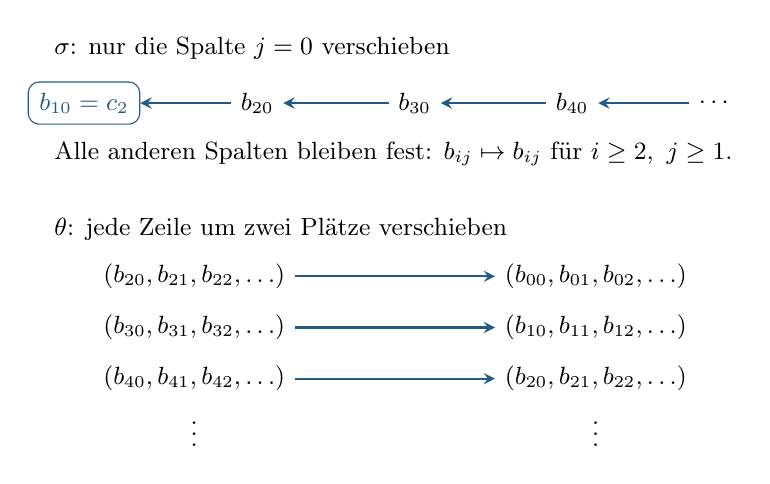
\begin{tikzpicture}[x=1cm,y=1cm,font=\small,>=stealth]
    \node[anchor=west] at (0,.7) {\(\sigma\): nur die Spalte \(j=0\) verschieben};
    \node[draw=mogblue,rounded corners,inner sep=4pt,text=mogblue] (s1) at (.5,0) {\(b_{10}=c_2\)};
    \node (s2) at (2.7,0) {\(b_{20}\)};
    \node (s3) at (4.7,0) {\(b_{30}\)};
    \node (s4) at (6.7,0) {\(b_{40}\)};
    \node (s5) at (8.5,0) {\(\cdots\)};
    \draw[->,thick,mogblue] (s2)--(s1);
    \draw[->,thick,mogblue] (s3)--(s2);
    \draw[->,thick,mogblue] (s4)--(s3);
    \draw[->,thick,mogblue] (s5)--(s4);
    \node[anchor=west] at (0,-.65)
      {Alle anderen Spalten bleiben fest: \(b_{i j}\mapsto b_{i j}\) für \(i\geq2,\ j\geq1\).};
    \node[anchor=west] at (0,-1.6) {\(\theta\): jede Zeile um zwei Plätze verschieben};
    \node (t20) at (1.9,-2.2) {\((b_{20},b_{21},b_{22},\ldots)\)};
    \node (t00) at (7,-2.2) {\((b_{00},b_{01},b_{02},\ldots)\)};
    \node (t30) at (1.9,-2.85) {\((b_{30},b_{31},b_{32},\ldots)\)};
    \node (t10) at (7,-2.85) {\((b_{10},b_{11},b_{12},\ldots)\)};
    \node (t40) at (1.9,-3.5) {\((b_{40},b_{41},b_{42},\ldots)\)};
    \node (t21) at (7,-3.5) {\((b_{20},b_{21},b_{22},\ldots)\)};
    \draw[->,thick,mogblue] (t20)--(t00);
    \draw[->,thick,mogblue] (t30)--(t10);
    \draw[->,thick,mogblue] (t40)--(t21);
    \node at (1.9,-4.1) {\(\vdots\)};
    \node at (7,-4.1) {\(\vdots\)};
  \end{tikzpicture}
  \par\smallskip\small\raggedright
  Jeder Pfeil zeigt vom Urbild zum Bild. Bei \(\sigma\) kommt genau
  der Punkt \(c_2\) zum Zielbereich hinzu; \(\theta\) trifft alle Zeilen von \(D\).
  \end{minipage}\par\medskip
}

\newcommand{\MogAbsorptionDiagram}{%
  \par\medskip\noindent
  \begin{minipage}{\linewidth}
  \centering
  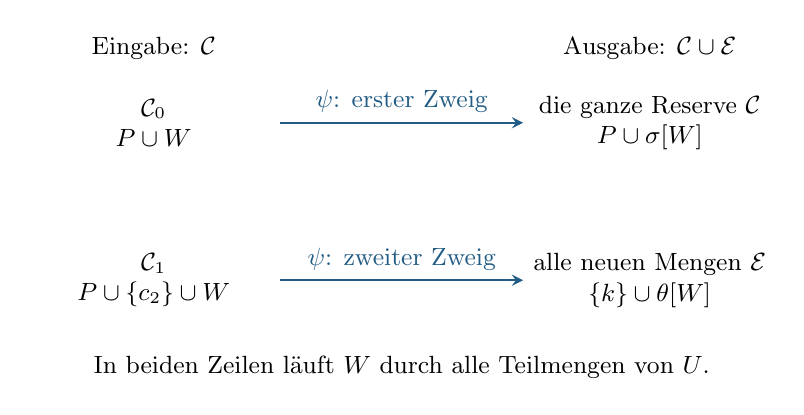
\begin{tikzpicture}[x=1cm,y=1cm,font=\small,>=stealth,
    family/.style={
      minimum width=3.2cm,minimum height=1.25cm,align=center}]
    \node at (0,.95) {Eingabe: \(\mathcal C\)};
    \node at (6.3,.95) {Ausgabe: \(\mathcal C\cup\mathcal E\)};
    \node[family] (c0) at (0,0) {\(\mathcal C_0\)\\\(P\cup W\)};
    \node[family] (c1) at (0,-2) {\(\mathcal C_1\)\\\(P\cup\{c_2\}\cup W\)};
    \node[family] (c) at (6.3,0) {die ganze Reserve \(\mathcal C\)\\\(P\cup\sigma[W]\)};
    \node[family] (e) at (6.3,-2) {alle neuen Mengen \(\mathcal E\)\\\(\{k\}\cup\theta[W]\)};
    \draw[->,thick,mogblue] (c0)--node[above,align=center] {\(\psi\): erster Zweig}(c);
    \draw[->,thick,mogblue] (c1)--node[above,align=center] {\(\psi\): zweiter Zweig}(e);
    \node[align=center] at (3.15,-3.1) {In beiden Zeilen läuft \(W\) durch alle Teilmengen von \(U\).};
  \end{tikzpicture}
  \par\smallskip\small\raggedright
  Die beiden Eingabefamilien sind disjunkt, ebenso die beiden Ausgabefamilien.
  Der obere Zweig füllt bereits die gesamte alte Reserve;
  der untere schafft Platz für sämtliche neuen \(k\)-haltigen Mengen in \(D\cup\{k\}\).
  \end{minipage}\par\medskip
}
